\documentclass[10pt,a4paper,twocolumn]{article}
\usepackage[utf8]{inputenc}

%PNAS fonts
\usepackage{mathptmx}
\usepackage{tgheros}

\usepackage{amssymb}
\usepackage[separate-uncertainty = true,multi-part-units=single]{siunitx}
\usepackage{multirow}
\usepackage{textcomp}

\usepackage{graphicx}

\usepackage{tikz}
\usetikzlibrary{calc, positioning, intersections, matrix, patterns}

\tikzset{lab/.style={above right, inner sep=0, font=\sffamily\Large\bfseries}}

\usepackage{pgfplots}
\usepgfplotslibrary{groupplots}

\pgfplotsset{compat=1.3, every axis/.append style={thick, mark size={0.2em}}}

\definecolor{Main}{rgb}{1, 0.57, 0}
\definecolor{Accent1}{rgb}{1,0.28,0}
\definecolor{Accent2}{rgb}{1,0.74,0}


\author{Mathieu Leocmach}
\begin{document}

\begin{figure}
	\begin{tikzpicture}
	\begin{axis}[%
		name=pH,
		xmin=0,xmax=8,
		ymin=0, ymax=7,
		xlabel={time (h)}, ylabel={\textcolor{Accent1}{pH}},
		extra tick style={grid=major},%
		extra y ticks={4.6}, extra y tick labels={},%
		%extra x ticks={0.55, 0.64, 0.72, 0.80, 1, 1.27, 2.5}, extra x tick labels={},%
		axis y line*=left,
		width=0.925\columnwidth,
		height=0.5\columnwidth,
		]
	\addplot+[no marks,Accent1] table[x expr={\thisrowno{0}/3600.+0.05}]{Y189_28800s.pH};
	%\node[base left=0] at (axis cs:8,4.6) {isoelectric};
	\end{axis}
	\begin{axis}[%
		xmin=0,xmax=8,
		ymin=0,
		ylabel=\textcolor{Main}{$G^\prime$ (\si{\pascal})},
		axis y line*=right,
		axis x line=none,
		width=0.925\columnwidth,
		height=0.5\columnwidth,
		]
	\addplot+[no marks,Main] table[x expr={\thisrowno{0}/3600.+0.05}]{Y235_28800s.prise};
	\end{axis}
	\node[lab, yshift=0.5em] at (pH.outer south west) {a};
	\begin{scope}[shift=(pH.outer south west), yshift=-2em]
		\fill[pattern=north east lines,pattern color=Accent2] (0,0) rectangle (\columnwidth,1.5em) node[midway,fill=white,inner sep=1pt] (glabeltop) {glass};
		\fill[pattern=north east lines,pattern color=Accent2] (0,-2.5em) rectangle (\columnwidth,-4em) node[midway,fill=white,inner sep=1pt] {glass};
		%acrylamide
		\begin{scope}[Accent1]
			\draw[line width=2pt] (0.05\columnwidth,-2.5em) -- (0.95\columnwidth,-2.5em) (0.05\columnwidth,-1pt) -- (0.95\columnwidth,-1pt);
			\node[inner sep=1pt, anchor=west] at (0.05\columnwidth,-1.25em) (brushlabel) {acrylamide brush};
			\draw[->,thick] (brushlabel.base) -- +(0,-0.8em);
			\draw[->,thick] (brushlabel.north) -- +(0,+0.4em);
		\end{scope}
		%spacer
		\begin{scope}[gray]
			\fill (0,0) rectangle (0.05\columnwidth,-2.5em) (\columnwidth,0) rectangle (0.95\columnwidth,-2.5em);
			\node[above left=0] at (\columnwidth,1.5em) (spacerlabel){spacer};
			\draw[->,thick] (spacerlabel.base) -- (0.975\columnwidth,1pt);
		\end{scope}
		%
		\draw[<->] (0.75\columnwidth,-2pt) -- (0.75\columnwidth,-2.5em) node[midway,left] {$e\sim \SI{100}{\micro\metre}$};
		\draw[<->] (0.05\columnwidth,-4.25em) -- (0.95\columnwidth,-4.25em) node[midway,below] (L) {$L\sim\SI{2}{\centi\metre}$};
		\node[lab] at (0,0 |- L.base) {b};
	\end{scope}
	%pictures
	\begin{scope}[inner sep=0, shift=(pH.outer south west), yshift=-8em]
		\node[anchor=north west] (a) {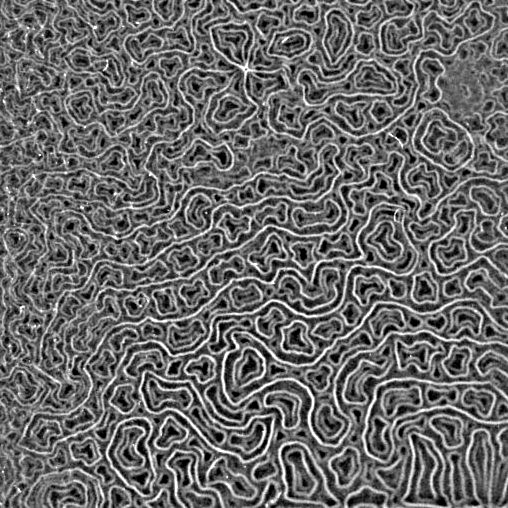
\includegraphics[width=0.28\columnwidth]{cas3p2_fluo0p8_GDL4_50um_coating_2_zoom2_crop}};
		\node[anchor=north] at (0.44\columnwidth,0) (b) {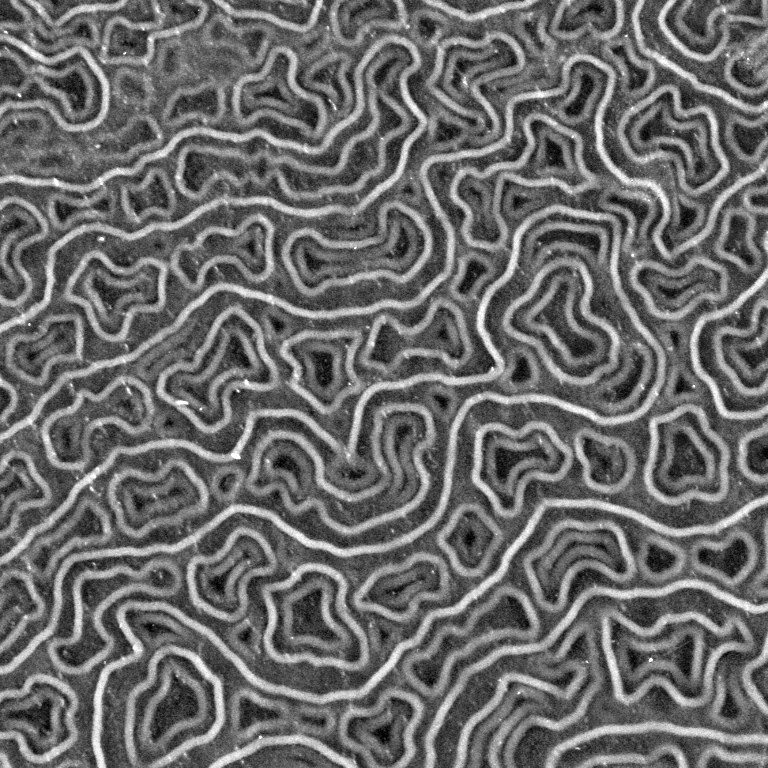
\includegraphics[width=0.28\columnwidth]{cas3p2_fluo0p8_GDL4_50um_coating_2_zoom6_crop}};
		\node[anchor=north east] at (\columnwidth,0) (c) {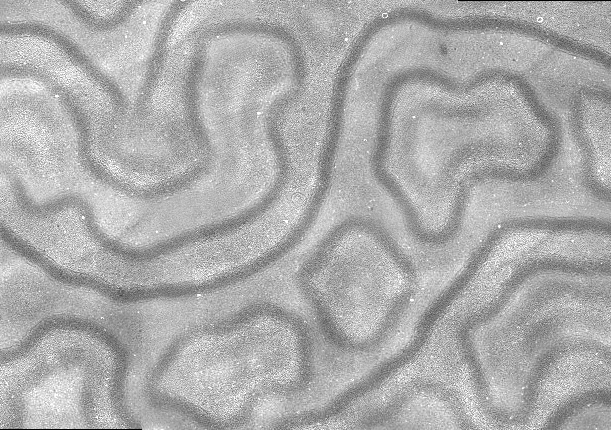
\includegraphics[width=0.4\columnwidth]{cas3p2_fluo0p8_GDL4_50um_coating_2_transmission}};
		%zooms
		\node[minimum width = 0.137\columnwidth, minimum height=0.137\columnwidth, anchor=north west, draw=Accent2] at ($(a.north west) +(0.111\columnwidth,-0.072\columnwidth)$) (bz){};
		\draw[Accent2] (bz.north east) -- (b.north west) (bz.south east) -- (b.south west);
		\node[minimum width = 0.128\columnwidth, minimum height=0.081\columnwidth, anchor=north west, draw=Main] at ($(b.north west) +(0.097\columnwidth,-0.143\columnwidth)$) (cz){};
		\draw[Main] (cz.north east) -- (c.north west) (cz.south east) -- (c.south west);
		\node[minimum width = 0.156\columnwidth, minimum height=0.156\columnwidth, anchor=north west, draw=Accent1] at ($(c.north west) + (0.125\columnwidth,0)$) (dz) {};
		%scale bars
		\draw[ultra thick] (a.south east) ++(0,-0.25em) -- ++(-0.178\columnwidth,0) node[pos=0.5, below=0.25em, font=\small] (M) {\SI{1}{\centi\metre}};
		\draw[ultra thick] (b.south east) ++(0,-0.25em) -- ++(-0.176\columnwidth,0) node[pos=0.5, below=0.25em, font=\small] {\SI{5}{\milli\metre}};
		\draw[ultra thick] (c.south east) ++(0,-0.25em) -- ++(-0.132\columnwidth,0) node[pos=0.5, below=0.25em, font=\small] {\SI{1}{\milli\metre}};
	\node[lab] at (0,0 |- M.base) {c};
	\node[lab] at (b.west |- M.base) {d};
	\node[lab] at (c.west |- M.base) {e};
	\end{scope}
	\end{tikzpicture}
	\caption{Acid induced gel. (a) Evolution of the pH and of the storage modulus with sticky boundary conditions. Horizontal line is the isoelectric pH. (b) Sketch of the cell with no adhesion of the protein on the top and bottom plates. (c-e) Resulting patterns in the same sample ($e=\SI{100}{\micro\metre}$) at different magnification by (c-d) reflexion or (e) transmission optical microscopy (tiled).}
	\label{fig:acidgel}
\end{figure}

\begin{figure*}
	\begin{tikzpicture}
	\matrix[matrix of nodes, inner sep=0, column sep=0.015\textwidth, row sep=0.5em] (m){
	33 min & 38 min & 43 min & 48 min & 1h & 1h15 & 2h30\\
	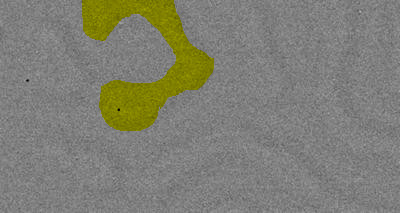
\includegraphics[width=0.13\textwidth]{prise_0100_color.jpg}&
	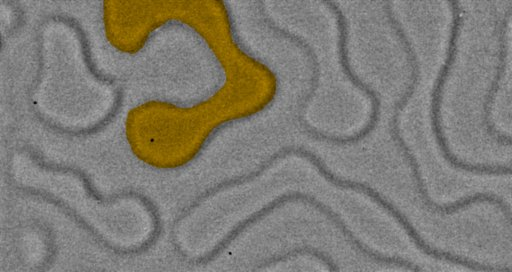
\includegraphics[width=0.13\textwidth]{prise_0130_color.jpg}&
	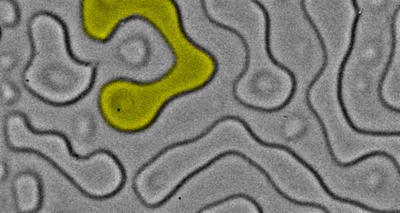
\includegraphics[width=0.13\textwidth]{prise_0160_color.jpg}&
	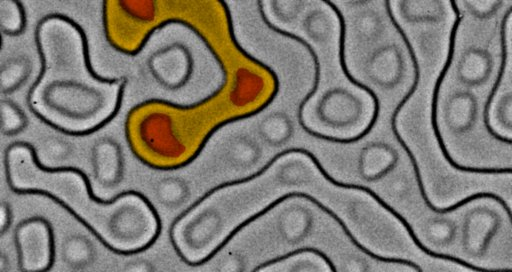
\includegraphics[width=0.13\textwidth]{prise_0190_color.jpg}&
	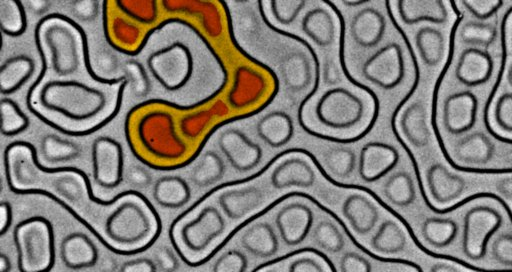
\includegraphics[width=0.13\textwidth]{prise_0250_color.jpg}&
	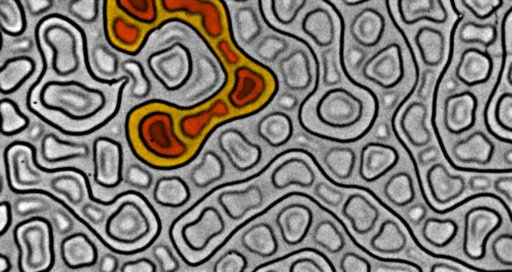
\includegraphics[width=0.13\textwidth]{prise_0360_color.jpg}&
	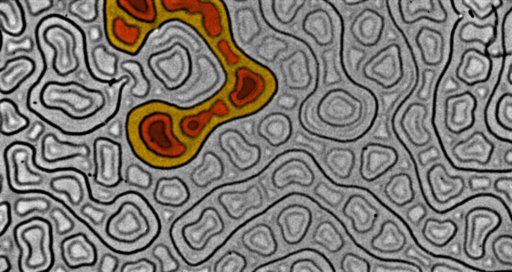
\includegraphics[width=0.13\textwidth]{prise_0799_color.jpg}\\
	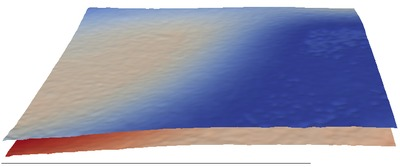
\includegraphics[width=0.13\textwidth]{cas3p2_fluo0p8_GDL4_2_t047_crop_resized.jpg}&
	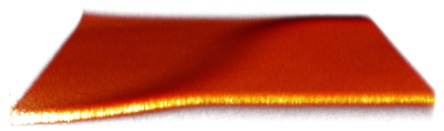
\includegraphics[width=0.13\textwidth]{cas3p2_fluo0p8_GDL4_2_t056_crop_resized.jpg}&
	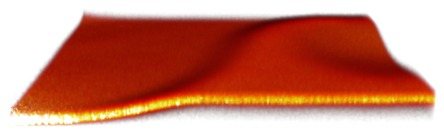
\includegraphics[width=0.13\textwidth]{cas3p2_fluo0p8_GDL4_2_t065_crop_resized.jpg}&
	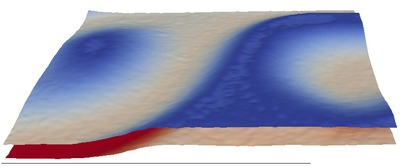
\includegraphics[width=0.13\textwidth]{cas3p2_fluo0p8_GDL4_2_t074_crop_resized.jpg}&
	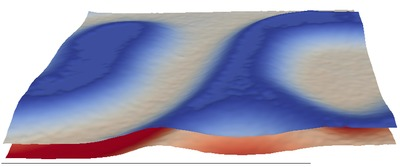
\includegraphics[width=0.13\textwidth]{cas3p2_fluo0p8_GDL4_2_t092_crop_resized.jpg}&
	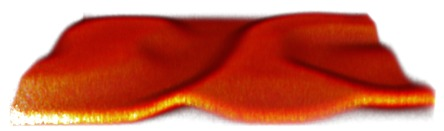
\includegraphics[width=0.13\textwidth]{cas3p2_fluo0p8_GDL4_2_t125_crop_resized.jpg}&
	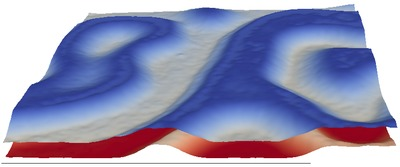
\includegraphics[width=0.13\textwidth]{cas3p2_fluo0p8_GDL4_2_t260_crop_resized.jpg}\\
	};
	\draw[ultra thick] ++(m-2-1.south west) -- ++(0.023\textwidth,0);
	\draw[ultra thick] ++(m-3-1.south west) -- ++(0.1\textwidth,0);
	\end{tikzpicture}
	\caption{Dynamics of pattern formation for $e\approx\SI{100}{\micro\metre}$. (top) By light transmission microscopy. (bottom) Reconstructed from fluorescent confocal microscopy (corresponds to the squared area in Fig.~\ref{fig:acidgel}e). Scale bars are \SI{1}{\milli\metre}.}
	\label{fig:dynamics}
\end{figure*}

\begin{figure}
	\begin{tikzpicture}
	\matrix[matrix of nodes, inner sep=0, column sep=0.01\columnwidth, row sep=0.01\columnwidth] (m) {
		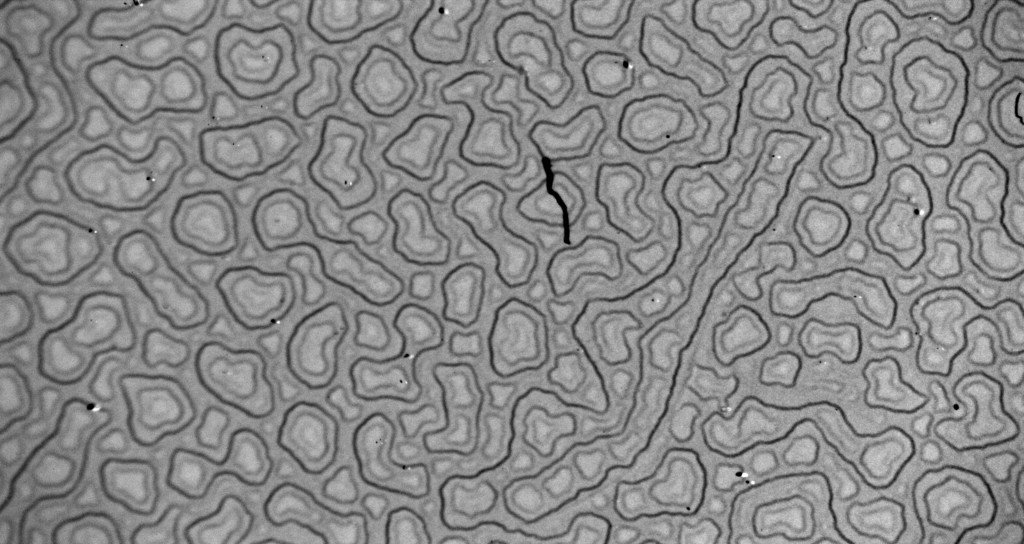
\includegraphics[width=0.245\columnwidth]{pattern_50um.jpg}&
		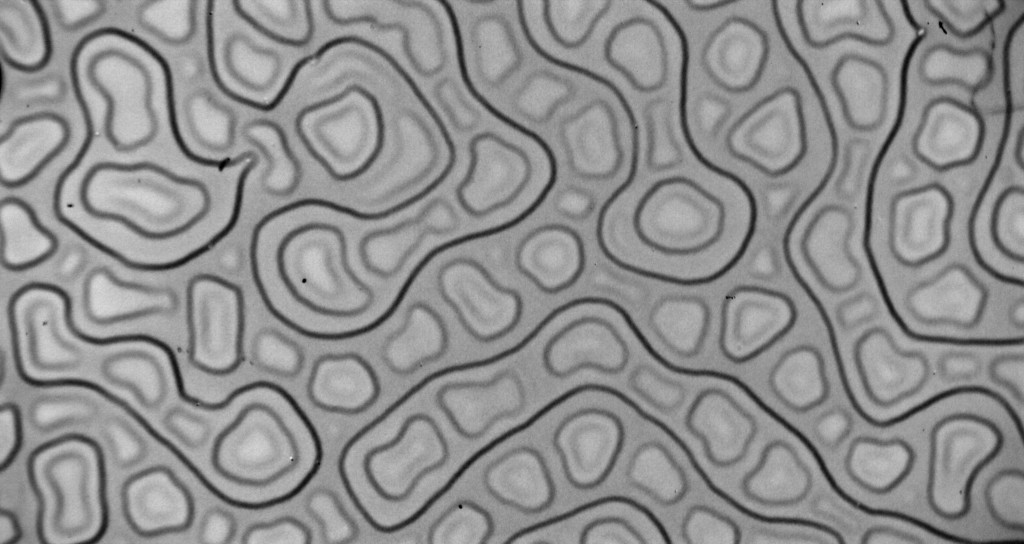
\includegraphics[width=0.245\columnwidth]{pattern_100um.jpg}&
		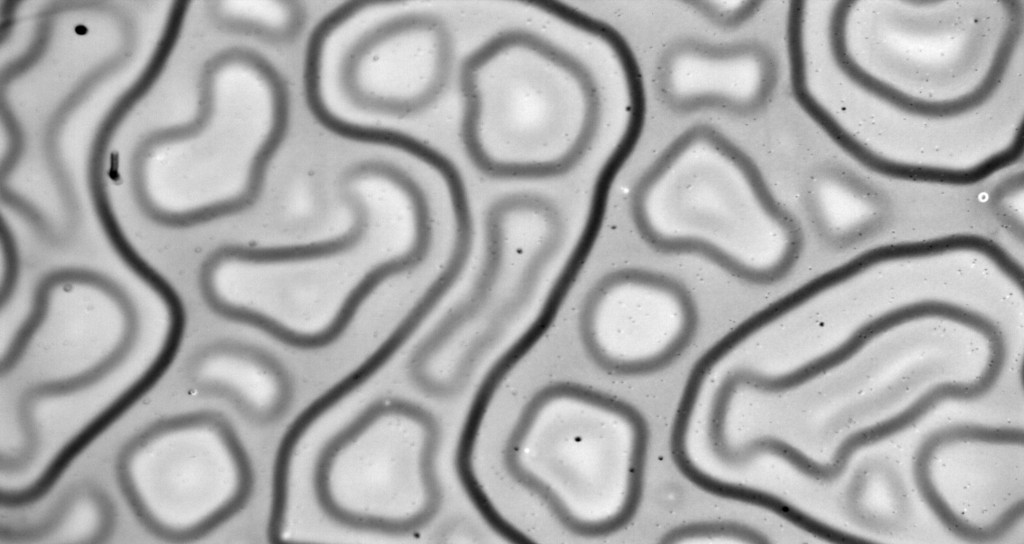
\includegraphics[width=0.245\columnwidth]{pattern_250um.jpg}&
		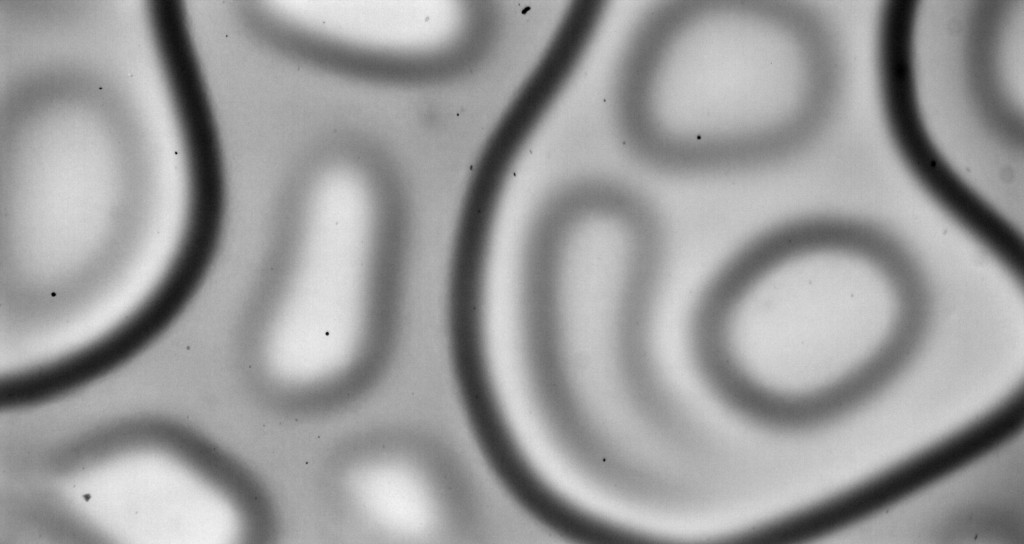
\includegraphics[width=0.245\columnwidth]{pattern_450um.jpg}\\
	};
	\node[inner sep=0, below left=0.01\columnwidth and 0 of m.south east] (x800) {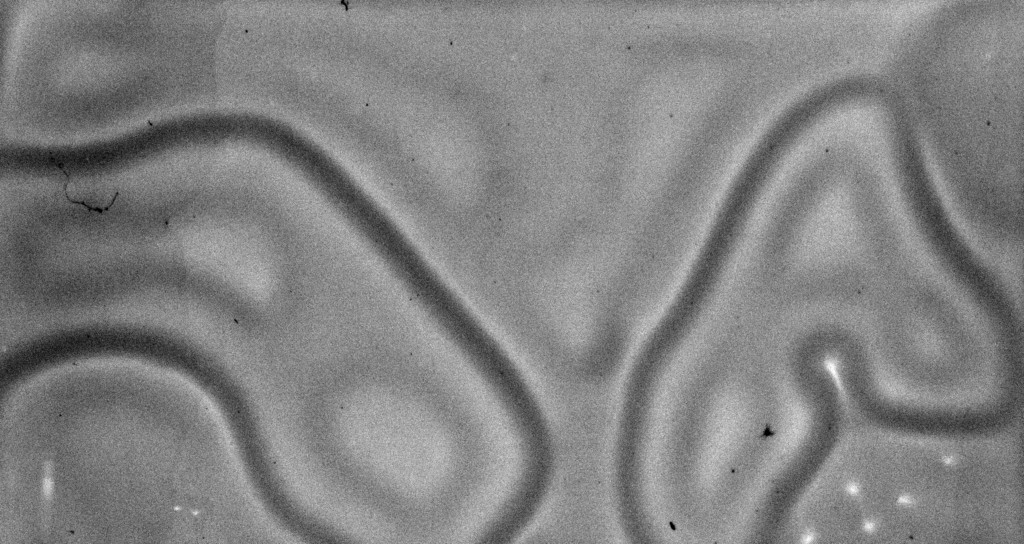
\includegraphics[width=0.49\columnwidth]{pattern_800um_x1.jpg}};
	\draw[ultra thick, Accent2, <->] (x800.south west) ++(0.196\columnwidth, 0.05\columnwidth) -- ++(0.145\columnwidth,0) node[midway,above]{$\lambda$};
	\draw[ultra thick,Main](x800.north east) -- ++(-0.217\columnwidth,0) node[midway,below] {\SI{5}{\milli\metre}};
	
	\begin{axis}[%
		name=g,
		anchor=left of north west,
		at={($(m.south west)+(0,-0.01\columnwidth)$)},
		scale only axis,
		width=0.4\columnwidth,
		height=0.175\columnwidth,
		xmin=0,xmax=1,xlabel={gap (\si{\milli\metre})},
		xtick={0,0.4,...,0.9},
		ymin=0,ylabel={$\lambda$ (\si{\milli\metre})},
		label shift=-0.5em,
		cycle multi list={%
			Accent1,no marks\\%
			Accent1,only marks,every mark/.append style={fill=Accent1},mark=*\\%
			Accent1,only marks,every mark/.append style={fill=white},mark=*\\%
			Accent1,only marks,every mark/.append style={fill=Accent1},mark=triangle*\\%
			Accent1,only marks,every mark/.append style={fill=white},mark=triangle*\\%
			Accent1,only marks,every mark/.append style={fill=Accent1},mark=square*\\%
			Accent1,only marks,every mark/.append style={fill=white},mark=square*\\%
		}
		]
		\addplot+[domain=0:3] {4.23*x};
		\addplot coordinates {(0.05,0.261)};\label{pgfplots:50}
		\addplot coordinates {(0.1,0.458)};\label{pgfplots:100}
		\addplot coordinates {(0.250,0.916)};\label{pgfplots:250}
		\addplot coordinates {(0.450,2.075)};\label{pgfplots:450}
		\addplot coordinates {(0.800,3.333)};\label{pgfplots:800}
		%\addplot+[only marks,Accent1, mark options={fill=Accent1}] coordinates {(0.05,0.261) (0.1,0.458) (0.250,0.916) (0.450,2.075) (0.800,3.333)};
	\end{axis}
	\node[below right=0 of m-1-1.north west] {\ref{pgfplots:50}};
	\node[below right=0 of m-1-2.north west] {\ref{pgfplots:100}};
	\node[below right=0 of m-1-3.north west] {\ref{pgfplots:250}};
	\node[below right=0 of m-1-4.north west] {\ref{pgfplots:450}};
	\node[below right=0 of x800.north west] {\ref{pgfplots:800}};
	\end{tikzpicture}
	\caption{Cell thickness dependence of the patterns. Each transmission microscopy picture corresponds to a point on the graph. Scale bar is common for all pictures.}
	\label{fig:thickness}
\end{figure}

\begin{figure}
	\begin{tikzpicture}
	\begin{groupplot}[%
		group style={
			group name=g, group size=1 by 3,
			xticklabels at=edge bottom,
			vertical sep=0,
			},
		xmin=0, xmax=200, xtick={0,30,...,180},
		extra tick style={grid=major},%
		extra x tick labels={},%
		width=1.03\columnwidth,
		height=0.5\columnwidth,
		]
	\nextgroupplot[ylabel={Position (\%)}, ymin=0, ymax=100]
	\addplot+[no marks,Accent1] table[y expr={\thisrowno{1}*100}]{mean_alt_rel_half_cas8.txt};
	\addplot+[only marks,Accent2, mark=+] table[y expr={\thisrowno{1}*100}]{mean_alt_rel_half_cas8_toi.txt};
	\node[lab,below left=0.2em] at (rel axis cs:1,1) {a};
	
	\nextgroupplot[ylabel={Volume (\%)}, ymin=20, ymax=100, extra x ticks={12.55}]
	\addplot+[no marks,Accent1] table[y expr={\thisrowno{1}*100}]{volume_rel_half_cas8.txt};
	\addplot+[only marks,Accent2, mark=+] table[y expr={\thisrowno{1}*100}]{volume_rel_half_cas8_toi.txt};
	\node[rotate=90, anchor=base east] at (axis cs:12.55,100) (syn) {synæresis};
	\node[above right=0 of syn.south west] {swelling};
	\node[lab,below left=0.2em] at (rel axis cs:1,1) {b};
	
	\nextgroupplot[ylabel={Excess area (\%)}, ymin=0, ymax=1.2, xlabel={time (min)}, extra x ticks={26.2, 42.8}]
	\addplot+[no marks,Accent1] table{excess_area_pc_half_cas8.txt};
	\addplot+[only marks,Accent2, mark=+] table{excess_area_pc_half_cas8_toi.txt};
	\node at (axis cs:13.35,1) {flat};
	\node[rotate=90, anchor=east] at (axis cs:34.75,1) {wrinkling};
	\node[anchor=west] at (axis cs:45,0.25) {wrinkling and buckling};
	\node[lab,above left=0.2em] at (rel axis cs:1,0) (c) {c};
	\coordinate (wr1) at (axis cs:26.2,0);
	\coordinate (wr2) at (axis cs:42.8,0);
	\end{groupplot}
	
	\begin{semilogyaxis}[
		name={zoom},
		at={(g c1r3.below south west)},
		anchor=above north west,
		width=0.5\columnwidth,
		height=0.6\columnwidth,
		xmin=26.2, xmax=42.8, xtick={25,30,...,180},
		ylabel={Excess area (\textperthousand)}, ymin=0.06, ymax=5,
		xlabel={time (min)},
		ytickten={-1,0}, yticklabels={0.1,1},
		]
		\addplot+[only marks,Accent1, mark=o] table[y expr={\thisrowno{1}*10}]{excess_area_pc_half_cas8.txt};
		\addplot+[only marks,Accent2, mark=+] table[y expr={\thisrowno{1}*10}]{excess_area_pc_half_cas8_toi.txt};
		\addplot+[black, no marks,domain=25:32.5] {10*exp(x/2.71-14.6)};
		\addplot+[black, no marks,domain=25:45] {10*exp(x/5.60-8.81)};
		\node[lab,above left=0.2em] at (rel axis cs:1,0) (d) {d};
	\end{semilogyaxis}
	\draw[help lines] (wr1)--(zoom.north west);
	\draw[help lines] (wr2)--(zoom.north east);
	
	\matrix[matrix of nodes, matrix anchor=north east, inner sep=0, column sep=0.02\textwidth, row sep=2pt] at (g c1r3.outer south east) (m){
	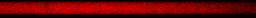
\includegraphics[width=0.48\columnwidth]{coupe_av10_cas8_t000.png}\\
	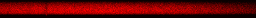
\includegraphics[width=0.48\columnwidth]{coupe_av10_cas8_t006.png}\\
	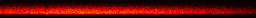
\includegraphics[width=0.48\columnwidth]{coupe_av10_cas8_t008.png}\\
	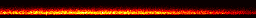
\includegraphics[width=0.48\columnwidth]{coupe_av10_cas8_t010.png}\\
	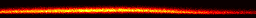
\includegraphics[width=0.48\columnwidth]{coupe_av10_cas8_t012.png}\\
	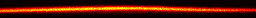
\includegraphics[width=0.48\columnwidth]{coupe_av10_cas8_t014.png}\\
	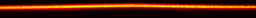
\includegraphics[width=0.48\columnwidth]{coupe_av10_cas8_t023.png}\\
	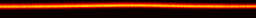
\includegraphics[width=0.48\columnwidth]{coupe_av10_cas8_t049.png}\\
	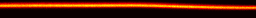
\includegraphics[width=0.48\columnwidth]{coupe_av10_cas8_t051.png}\\
	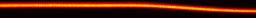
\includegraphics[width=0.48\columnwidth]{coupe_av10_cas8_t053.png}\\
	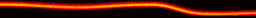
\includegraphics[width=0.48\columnwidth]{coupe_av10_cas8_t078.png}\\
	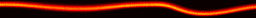
\includegraphics[width=0.48\columnwidth]{coupe_av10_cas8_t088.png}\\
	};
	%\draw[>->,gray,ultra thick] (m-2-1.east) -- (m-7-1.east) -- (m-2-2.west) -- (m-7-2.west);
	\node[lab,anchor=base east] at (m-1-1.north -| c.east) {e};
	
	%\node[inner sep=0, anchor=south east] (g-1-1.outer north west){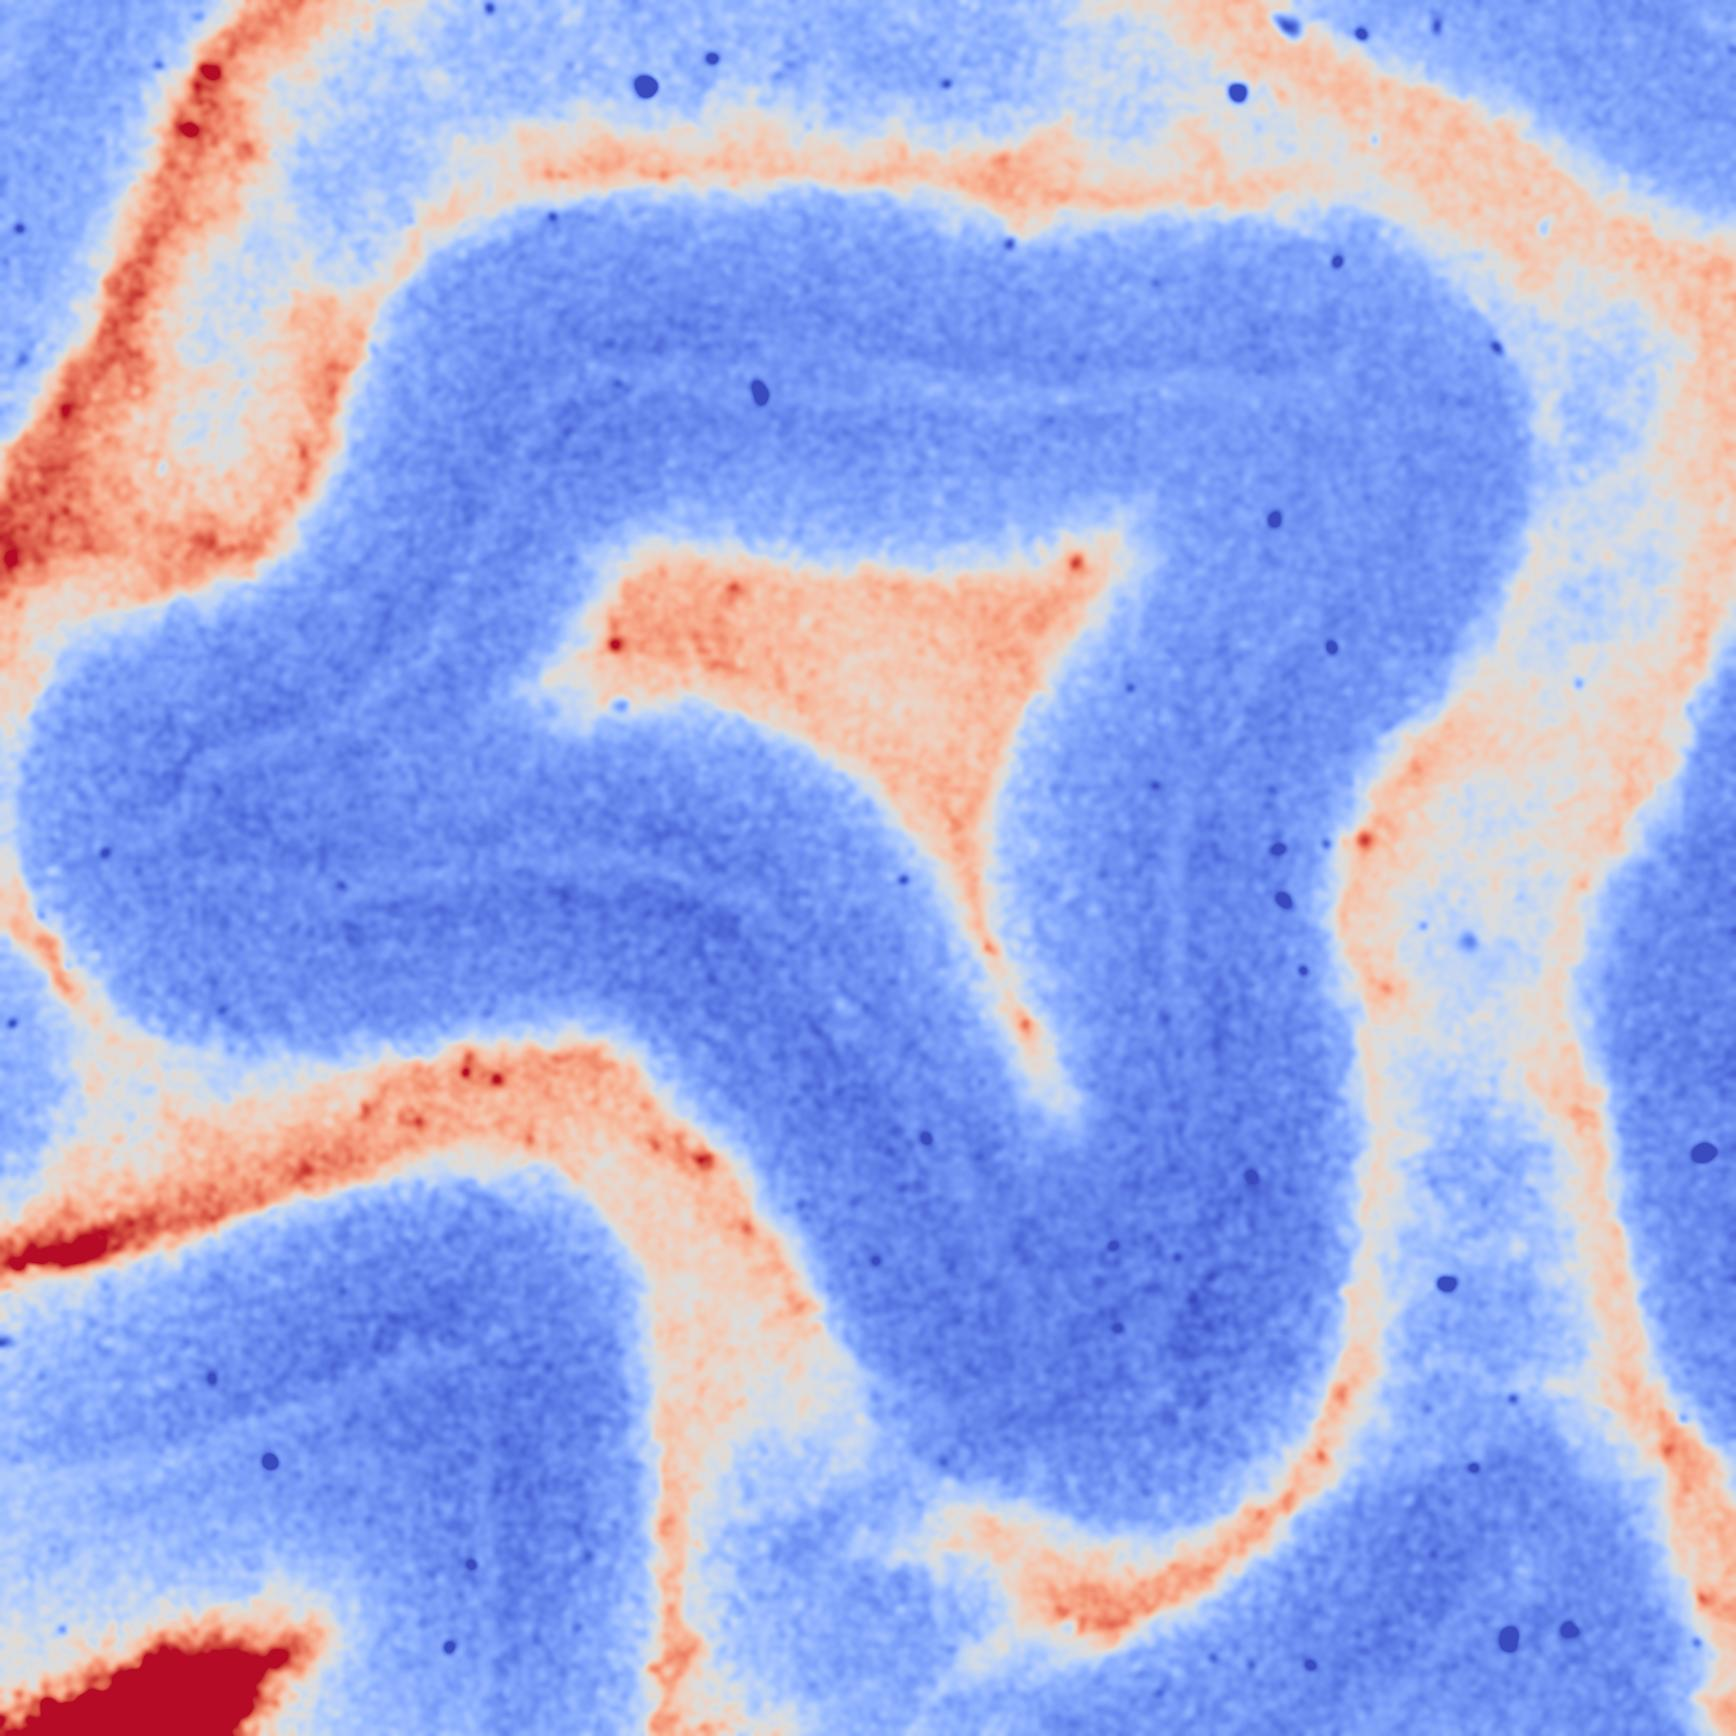
\includegraphics[width=0.45\columnwidth]{plastic_confocal}};
	\end{tikzpicture}
	\caption{Synæresis and swelling, cas. 8\%, GDL 7.2\% (a) Average relative altitude, (b) volume (c-d) midsurface area of the gel phase. Straight lines are exponential fits with time constants \SI{170 \pm 7}{\second} and \SI{337 \pm 3}{\second}. (e) Successive confocal XZ slices (field of view is $1\times\SI{0.1}{\milli\metre}$), colors indicate the protein concentration. Times of the snapshots are marked as crosses on (a-d). Note that swelling starts \SI{14}{\minute} before wrinkling. The thickness increase is $\approx\SI{0.2}{px}$, thus not directly visible on the pictures.}
	\label{fig:wrinkles}
\end{figure}

\end{document}